\documentclass[11pt]{article}
\usepackage[toc,page]{appendix}
\usepackage{amsmath, amssymb}
\usepackage[utf8]{inputenc} % Already loaded below, technically redundant but harmless
\usepackage[T1]{fontenc}    % Already loaded below, technically redundant but harmless
\usepackage[style=apa,backend=biber]{biblatex}
%\usepackage{biblatex} % Commented out as biblatex is loaded above with options
\addbibresource{references.bib}
\usepackage{graphicx}
\usepackage{tikz}
\usetikzlibrary{automata,positioning,shapes.geometric, arrows.meta, fit, backgrounds, calc, chains}
\graphicspath{./images/Easy_Pictures/SMR_MULT_Repackaging}%\usepackage{kpfonts}
\usepackage{float}
\usepackage[margin=1in]{geometry}
\usepackage{cancel}
\usepackage{epsfig} % Note: `graphicx` is generally preferred over `epsfig` nowadays
\usepackage{tikz-3dplot}
\usepackage{darkmode} % Ensure this works well with listings colors if you enable it
\usepackage{dirtytalk}
\usepackage{longtable,booktabs,array}
\usepackage{calc} % for calculating minipage widths
\usepackage[utf8]{inputenc}
\usepackage[T1]{fontenc}
\usepackage{xcolor} % Needed for colors in listings
\usepackage{listings} % The core package for code listings

\usepackage{etoolbox}
\usepackage{hyperref}
\hypersetup{
 colorlinks=true,
 linkcolor=blue,
 filecolor=magenta,
 urlcolor=cyan,
 pdftitle={Hermeneutic Calculator},
 citecolor=blue,
 }
\urlstyle{same}

% --- Python Listings Setup ---
\definecolor{codegreen}{rgb}{0,0.6,0}  % Green for comments
\definecolor{codegray}{rgb}{0.5,0.5,0.5}    % Gray for line numbers
\definecolor{codepurple}{rgb}{0.58,0,0.82} % Purple for strings
\definecolor{backcolour}{rgb}{0.95,0.95,0.92} % Background color for code blocks

\lstdefinestyle{pythonStyle}{
    language=Python,                % Set language to Python
    backgroundcolor=\color{backcolour}, % Set background color
    commentstyle=\color{codegreen}\itshape, % Comment style (italic green)
    keywordstyle=\color{blue}\bfseries,    % Keyword style (bold blue)
    numberstyle=\tiny\color{codegray},    % Line number style (tiny gray)
    stringstyle=\color{codepurple},       % String style (purple)
    basicstyle=\ttfamily\small,     % Basic font style (small typewriter)
    breakatwhitespace=false,
    breaklines=true,                % Enable line breaking
    captionpos=b,                   % Caption position (bottom)
    keepspaces=true,                % Keep spaces to preserve indentation
    numbers=left,                   % Line numbers on the left
    numbersep=5pt,                  % Space between number and code
    showspaces=false,               % Don't show spaces as special characters
    showstringspaces=false,        % Don't show spaces in strings specially
    showtabs=false,                 % Don't show tabs as special characters
    tabsize=4,                      % Set tab size to 4 spaces
    frame=single,                   % Add a frame around the code
    rulecolor=\color{black},        % Frame color
    columns=fullflexible            % Ensure flexible columns
}

% Set the default style for all listings environments/commands
\lstset{style=pythonStyle}

% --- Removed/Commented Out HTML Specific Definitions ---
% \lstdefinestyle{htmlStyle}{ ... } % Removed
% \lstdefinelanguage{HTML}{ ... }  % Removed
% \lstset{style=htmlstyle, language=html} % Replaced by pythonStyle above

% Example of how to include a Python file (optional, uncomment and adjust path)
% \lstinputlisting[language=Python, caption={Example Python Script}]{./path/to/your/python_script.py}

% Optional: define some custom colors (already defined for listings above, keep if used elsewhere)
\definecolor{sliceRed}{RGB}{225,224,91} % matching "varyellow" from your code
\definecolor{linkYellow}{RGB}{255,215,0} % a golden yellow
\tdplotsetmaincoords{70}{110}

\title{Counting in Base 10}
\author{Theodore M. Savich}
\date{\today}

\begin{document}

\maketitle


\section{Diagonalizing the Count}\label{sec:diagonalizing_the_count}
\subsection{Sublation in Counting: From Tallies to Base Systems}\label{sublation-in-counting-from-tallies-to-base-systems}

Counting is not merely an accumulation of marks -- it is a process that both \textit{preserves} and \textit{transforms} prior determinations. In Hegelian terms, this movement is called \textit{sublation} (Aufhebung), the simultaneous \textit{negation}, \textit{preservation}, and \textit{uplift} of what came before. In mathematical practice, sublation is most clearly seen in the way base systems reorganize quantities into new structural units.

Consider a simple act of tally counting. If one were to count to nine using tally marks, the representation would appear as: 
\[
\vert\vert\vert\vert\vert\vert\vert\vert\vert
\]
Each tally stands independently as a discrete marker of a counted object that mirrors the ``world of ones'' reflected in von Neumann ordinals. They could just go on and on, accumulating indefinitely. While it is more normal to represent a transformation at 5 units, let us instead live in base ten. When ten is reached, the representation undergoes an important transformation:
\[
\cancel{\vert\vert\vert\vert\vert\vert\vert\vert\vert}
\]
The previous nine marks are not erased. They are not `gone.' But they are \textit{negated} and \textit{uplifted} into a new structural form. Out of the many ones, there is now one ten. This is a mathematical instance of sublation. The prior elements are not discarded. They are reorganized in a higher-level composition. The transition from loose tallies to a single ``ten'' does not merely introduce a new symbol; it alters how the prior marks are understood. They are still `present,' but they no longer function as isolated entities. 

So, using base systems involves ``two views'' of a number - but under the hood is very basic version of a diagonalizing function, $\delta$, that lets an element reference the whole system it’s part of. Ten loose ones is a "many", one 10 is a "one". Diagonalization is, therefore, a way of thinking about the problem of the one and the many. 


\section{Understanding the Recursive Nature of Counting}

Counting in base 10 involves incrementing digits and managing composition across multiple place values:
\begin{itemize}
    \item \textbf{Units (Ones):} $10^0 = 1$
    \item \textbf{Tens:} $10^1 = 10$
    \item \textbf{Hundreds:} $10^2 = 100$
    \item \textbf{Thousands:} $10^3 = 1,000$, etc.
\end{itemize}

The recursive process for counting follows these steps:
\begin{enumerate}
    \item Increment the units digit.
    \item If the units digit reaches 10, reset it to 0 and increment the tens digit.
    \item Repeat this process recursively for higher place values as needed.
\end{enumerate}

This recursive nature allows for counting indefinitely by reusing the same increment and composition logic for each digit.

\section{Why Use a Pushdown Automaton (PDA)?}

A Pushdown Automaton (PDA) is suitable for modeling recursive counting due to its ability to use a stack for memory. Here's why:
\begin{itemize}
    \item \textbf{Finite State Automaton (FSA):} Lacks the memory to handle arbitrary-length counts and composition.
    \item \textbf{Pushdown Automaton (PDA):} Uses a stack to provide additional memory, enabling nested operations like composition in counting.
    \item \textbf{Turing Machine:} While capable, it is more complex than needed for this task.
\end{itemize}

A PDA's stack can represent digit states and manage composition recursively, making it an appropriate choice.

\section{Designing a PDA for Three-Digit Base-10 Counting (0-999)} \label{sec:designing_3digit_pda}

While the unbounded recursive nature of counting presents challenges for standard PDA models, we can successfully design a PDA to handle counting within a fixed, practical range. This section details a Deterministic Pushdown Automaton (DPDA) capable of counting from 0 to 999, demonstrating how the stack and finite state control can manage multi-digit carries. This approach avoids the theoretical issues of infinite states or alphabets required by some conceptual models, providing a formally sound automaton for a three-digit counter.

\subsection{Simulating Three Digits on One Stack}
We represent the three place values (Hundreds, Tens, and Units) using distinct symbols on the PDA's single stack:
\begin{itemize}
    \item \textbf{Units Digit Symbols:} $U_0, U_1, \ldots, U_9$
    \item \textbf{Tens Digit Symbols:} $T_0, T_1, \ldots, T_9$
    \item \textbf{Hundreds Digit Symbols:} $H_0, H_1, \ldots, H_9$
\end{itemize}
A number, represented conventionally as $XYZ$ (X=Hundreds, Y=Tens, Z=Units), will be stored on the stack with the units digit on top. The stack configuration will be $(\#, H_X, T_Y, U_Z)$, where $\#$ is the bottom marker. For example, the number 123 would be represented by the stack $(\#, H_1, T_2, U_3)$.

\subsection{Components of the Three-Digit PDA}
The PDA is defined by the 7-tuple $M = (Q, \Sigma, \Gamma, \delta, q_{\text{start}}, \#, F)$:
\begin{itemize}
    \item \textbf{States ($Q$):} A finite set of states manages the counting and multi-level carry logic:
    \begin{enumerate}
        \item $q_{\text{start}}$: The initial state for setup.
        \item $q_{\text{idle}}$: The main state where the PDA resides when holding a valid count (0-999). This is the accepting state.
        \item $q_{\text{inc\_tens}}$: Intermediate state entered when the units digit rolls over ($U_9 \rightarrow U_0$), signaling the need to process the tens digit via an epsilon transition.
        \item $q_{\text{inc\_hundreds}}$: Intermediate state entered when the tens digit rolls over ($T_9 \rightarrow T_0$), signaling the need to process the hundreds digit via an epsilon transition.
        \item $q_{\text{halt}}$: A non-accepting state entered when an attempt is made to increment the count beyond 999 (hundreds digit rollover).
    \end{enumerate}
    \item \textbf{Input Alphabet ($\Sigma$):} Contains a symbol representing one unit to be counted, plus the empty string $\epsilon$ for internal transitions.
    \[ \Sigma = \{ \text{tick}, \epsilon \} \]
    \item \textbf{Stack Alphabet ($\Gamma$):} Includes the bottom marker and symbols for each digit in each place value.
    \[ \Gamma = \{ \#, H_0, \dots, H_9, T_0, \dots, T_9, U_0, \dots, U_9 \} \]
    \item \textbf{Transition Function ($\delta$):} Defined formally in Section~\ref{sec:formaltransition3digit}.
    \item \textbf{Initial State ($q_0$):} $q_{\text{start}}$.
    \item \textbf{Initial Stack Symbol ($Z_0$):} $\#$. (Implicitly placed on the stack at start).
    \item \textbf{Final States ($F$):} Only the state representing a valid count within the range is accepting.
    \[ F = \{ q_{\text{idle}} \} \]
\end{itemize}

\subsection{Automaton Behavior}
The three-digit counter operates as follows:
\begin{enumerate}
    \item \textbf{Initialization:} Start in $q_{\text{start}}$. On an epsilon transition seeing $\#$, push $H_0, T_0, U_0$ onto the stack (representing 0) and transition to $q_{\text{idle}}$. Stack: $(\#, H_0, T_0, U_0)$.
    \item \textbf{Counting (Units Increment):} In state $q_{\text{idle}}$, read a 'tick' input.
        \begin{itemize}
            \item If the top symbol is $U_n$ where $n < 9$, pop $U_n$, push $U_{n+1}$, and remain in $q_{\text{idle}}$.
            \item If the top symbol is $U_9$, pop $U_9$, push nothing. Transition to $q_{\text{inc\_tens}}$ to handle the carry to the tens place. The $T_Y$ symbol is now exposed on top.
        \end{itemize}
    \item \textbf{Carry Handling (Tens Increment):} In state $q_{\text{inc\_tens}}$, perform an epsilon transition based on the exposed tens digit $T_m$:
        \begin{itemize}
            \item If the top symbol is $T_m$ where $m < 9$, pop $T_m$. Push $T_{m+1}$, then push $U_0$. Transition back to $q_{\text{idle}}$. The carry is complete. Stack: $(\#, H_X, T_{m+1}, U_0)$.
            \item If the top symbol is $T_9$, pop $T_9$, push nothing. Transition to $q_{\text{inc\_hundreds}}$ to handle the carry to the hundreds place. The $H_X$ symbol is now exposed on top.
        \end{itemize}
    \item \textbf{Carry Handling (Hundreds Increment):} In state $q_{\text{inc\_hundreds}}$, perform an epsilon transition based on the exposed hundreds digit $H_k$:
        \begin{itemize}
            \item If the top symbol is $H_k$ where $k < 9$, pop $H_k$. Push $H_{k+1}$, then push $T_0$, then push $U_0$. Transition back to $q_{\text{idle}}$. The carry is complete. Stack: $(\#, H_{k+1}, T_0, U_0)$.
            \item If the top symbol is $H_9$ (representing an attempt to increment 999), pop $H_9$. Push $H_0$, then push $T_0$, then push $U_0$. Transition to the non-accepting state $q_{\text{halt}}$. Stack: $(\#, H_0, T_0, U_0)$.
        \end{itemize}
     \item \textbf{Halt State:} Once in $q_{\text{halt}}$, no further transitions are defined. The machine halts and implicitly rejects any further input, indicating overflow beyond 999.
\end{enumerate}

\section{State Diagram for Three-Digit Counter} \label{sec:state_diagram_3digit}

The diagram illustrates the states and key transitions. Multi-symbol stack operations are abbreviated (e.g., $T_m \rightarrow U_0, T_{m+1}$ means pop $T_m$, push $T_{m+1}$, push $U_0$).

\begin{figure}[H]
    \centering
    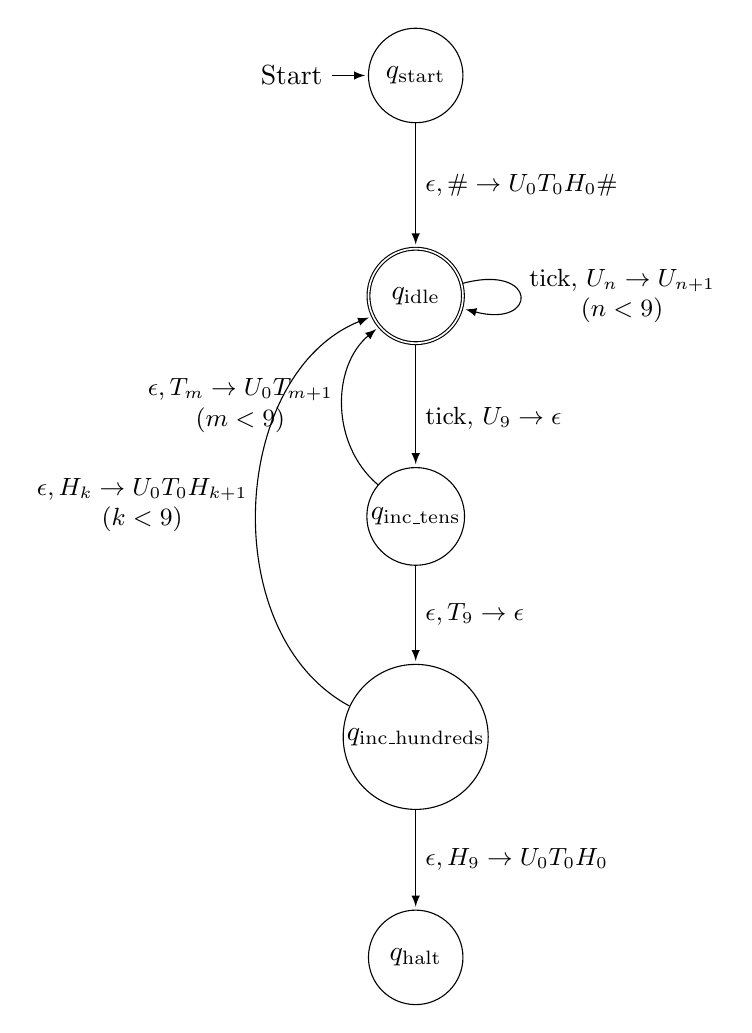
\begin{tikzpicture}[
        shorten >=1pt, 
        node distance=2.8cm, % Keep vertical distance
        on grid, 
        auto,
        >=latex, 
        state/.style={circle, draw, minimum size=1.2cm, inner sep=1pt}, 
        every edge/.style={draw, ->},
        label/.style={font=\small, align=center} % Consistent label style
      ]
        % Position nodes vertically
        \node[state, initial, initial text={Start}] (q_start) {$q_{\text{start}}$};
        \node[state, accepting, below=of q_start] (q_idle) {$q_{\text{idle}}$}; 
        \node[state, below=of q_idle] (q_inc_tens) {$q_{\text{inc\_tens}}$}; 
        \node[state, below=of q_inc_tens] (q_inc_hundreds) {$q_{\text{inc\_hundreds}}$}; 
        \node[state, below=of q_inc_hundreds] (q_halt) {$q_{\text{halt}}$}; 

        % Transitions going mostly downwards
        \path
        (q_start) edge node[right, label] {$\epsilon, \# \to U_0 T_0 H_0 \#$} (q_idle) 
        
        (q_idle) edge node[right, label, pos=0.6] {tick, $U_9 \to \epsilon$} (q_inc_tens) 
        
        (q_inc_tens) edge node[right, label] {$\epsilon, T_9 \to \epsilon$} (q_inc_hundreds)
        
        (q_inc_hundreds) edge node[right, label] {$\epsilon, H_9 \to U_0 T_0 H_0$} (q_halt) 
        
        % Loop on q_idle - POSITIONED TO THE RIGHT
        (q_idle) edge [loop right] node[label, right] {tick, $U_n \to U_{n+1}$\\ ($n<9$)} (q_idle) 
        
        % Return paths from carry states using bends
        (q_inc_tens) edge [bend left=50] node[left, label, pos=0.5] {$\epsilon, T_m \to U_0 T_{m+1}$ \\ ($m<9$)} (q_idle) 
        
        (q_inc_hundreds) edge [bend left=65] node[left, label, pos=0.5] {$\epsilon, H_k \to U_0 T_0 H_{k+1}$ \\ ($k<9$)} (q_idle); 
        
    \end{tikzpicture}
    \caption{State Diagram for the Three-Digit (0-999) Counter PDA}
\end{figure}

\section{Detailed Example Execution: Counting from 98 to 101} \label{sec:example_3digit}

This section demonstrates handling carries across two place values.

\begin{enumerate}
    \item \textbf{Start at 98:} Assume the PDA is in state $q_{\text{idle}}$ with stack $(\#, H_0, T_9, U_8)$.
    \item \textbf{Input 99 ('tick'):}
        \begin{itemize}
            \item In $q_{\text{idle}}$, reads 'tick'. Top is $U_8$. Pops $U_8$, pushes $U_9$. Stays $q_{\text{idle}}$.
            \item Stack: $(\#, H_0, T_9, U_9)$ (represents 99).
        \end{itemize}
    \item \textbf{Input 100 ('tick'):}
        \begin{itemize}
            \item In $q_{\text{idle}}$, reads 'tick'. Top is $U_9$. Pops $U_9$, pushes nothing. Enters $q_{\text{inc\_tens}}$.
            \item Stack: $(\#, H_0, T_9)$.
            \item Epsilon transition from $q_{\text{inc\_tens}}$. Top is $T_9$. Pops $T_9$, pushes nothing. Enters $q_{\text{inc\_hundreds}}$.
            \item Stack: $(\#, H_0)$.
            \item Epsilon transition from $q_{\text{inc\_hundreds}}$. Top is $H_0$. Pops $H_0$. Pushes $H_1$, then $T_0$, then $U_0$. Enters $q_{\text{idle}}$.
            \item Stack: $(\#, H_1, T_0, U_0)$ (represents 100).
        \end{itemize}
    \item \textbf{Input 101 ('tick'):}
        \begin{itemize}
            \item In $q_{\text{idle}}$, reads 'tick'. Top is $U_0$. Pops $U_0$, pushes $U_1$. Stays $q_{\text{idle}}$.
            \item Stack: $(\#, H_1, T_0, U_1)$ (represents 101).
        \end{itemize}
\end{enumerate}

\section{Handling Multi-Level Carries} \label{sec:carry_handling_3digit}

This PDA manages carries across multiple digits using intermediate states:
\begin{enumerate}
    \item \textbf{Units Carry:} $U_9$ rollover triggers a transition to $q_{\text{inc\_tens}}$, popping $U_9$ and exposing the tens digit $T_Y$.
    \item \textbf{Tens Processing:} $q_{\text{inc\_tens}}$ handles $T_Y$ via epsilon transition.
        \begin{itemize}
            \item If $Y < 9$, it increments $T_Y$ to $T_{Y+1}$, pushes the $U_0$, and returns control to $q_{\text{idle}}$.
            \item If $Y = 9$, it pops $T_9$ and transitions control to $q_{\text{inc\_hundreds}}$, exposing the hundreds digit $H_X$.
        \end{itemize}
    \item \textbf{Hundreds Processing:} $q_{\text{inc\_hundreds}}$ handles $H_X$ via epsilon transition.
        \begin{itemize}
            \item If $X < 9$, it increments $H_X$ to $H_{X+1}$, pushes $T_0$, pushes $U_0$, and returns control to $q_{\text{idle}}$.
            \item If $X = 9$, it pushes $H_0, T_0, U_0$ (representing the rollover part) and transitions to $q_{\text{halt}}$ to signal overflow.
        \end{itemize}
\end{enumerate}
This chained state transition correctly simulates the ripple effect of a carry across units, tens, and hundreds places.

\section{Formal Transition Function ($\delta$) for Three-Digit Counter} \label{sec:formaltransition3digit}

The transition function $\delta: Q \times (\Sigma \cup \{\epsilon\}) \times \Gamma \rightarrow Q \times \Gamma^*$ is defined as:
*(Note: Stack push $(S_1, S_2, \dots)$ pushes $S_n$ first, ..., $S_2$, then $S_1$ last/top)*

\begin{itemize}
    \item \textbf{Initialization:}
        \[ \delta(q_{\text{start}}, \epsilon, \#) = (q_{\text{idle}}, (U_0, T_0, H_0, \#)) \]
        
    \item \textbf{Idle State (Units):} For $n \in \{0, \ldots, 8\}$:
        \[ \delta(q_{\text{idle}}, \text{tick}, U_n) = (q_{\text{idle}}, (U_{n+1})) \]
        \[ \delta(q_{\text{idle}}, \text{tick}, U_9) = (q_{\text{inc\_tens}}, ()) \] % Pop U9
        
    \item \textbf{Tens Carry State (Epsilon):} For $m \in \{0, \ldots, 8\}$:
        \[ \delta(q_{\text{inc\_tens}}, \epsilon, T_m) = (q_{\text{idle}}, (U_0, T_{m+1})) \] % Pop Tm, Push T(m+1), Push U0
        \[ \delta(q_{\text{inc\_tens}}, \epsilon, T_9) = (q_{\text{inc\_hundreds}}, ()) \] % Pop T9
        
    \item \textbf{Hundreds Carry State (Epsilon):} For $k \in \{0, \ldots, 8\}$:
        \[ \delta(q_{\text{inc\_hundreds}}, \epsilon, H_k) = (q_{\text{idle}}, (U_0, T_0, H_{k+1})) \] % Pop Hk, Push H(k+1), T0, U0
        \[ \delta(q_{\text{inc\_hundreds}}, \epsilon, H_9) = (q_{\text{halt}}, (U_0, T_0, H_0)) \] % Pop H9, Push H0, T0, U0
        
    \item \textbf{Halt State:}
        \[ \delta(q_{\text{halt}}, \cdot, \cdot) = \emptyset \]
\end{itemize}

\section{Example: Counting from 998 to Overflow} \label{sec:example_overflow_3digit}

Tracing the behavior at the upper limit:
\begin{enumerate}
    \item \textbf{Start at 998:} State $q_{\text{idle}}$, Stack $(\#, H_9, T_9, U_8)$.
    \item \textbf{Input 999 ('tick'):}
        \begin{itemize}
            \item $\delta(q_{\text{idle}}, \text{tick}, U_8) = (q_{\text{idle}}, (U_9))$.
            \item Stack: $(\#, H_9, T_9, U_9)$ (represents 999). State $q_{\text{idle}}$.
        \end{itemize}
    \item \textbf{Input 1000 ('tick'):}
        \begin{itemize}
            \item $\delta(q_{\text{idle}}, \text{tick}, U_9) = (q_{\text{inc\_tens}}, ())$.
            \item Stack: $(\#, H_9, T_9)$. State $q_{\text{inc\_tens}}$.
            \item $\epsilon$-trans: $\delta(q_{\text{inc\_tens}}, \epsilon, T_9) = (q_{\text{inc\_hundreds}}, ())$.
            \item Stack: $(\#, H_9)$. State $q_{\text{inc\_hundreds}}$.
            \item $\epsilon$-trans: $\delta(q_{\text{inc\_hundreds}}, \epsilon, H_9) = (q_{\text{halt}}, (U_0, T_0, H_0))$.
            \item Stack: $(\#, H_0, T_0, U_0)$. State $q_{\text{halt}}$.
        \end{itemize}
    \item \textbf{State $q_{\text{halt}}$:} The PDA enters the non-accepting halt state. The stack represents '000', but the state signals the overflow. Further 'tick' inputs are rejected as no transitions are defined from $q_{\text{halt}}$.
\end{enumerate}

\section{Practical Considerations and Limitations} \label{sec:practical_considerations_3digit}

This three-digit counter PDA successfully models counting within its defined range (0-999).
\begin{itemize}
    \item \textbf{Bounded Range:} The automaton is explicitly designed for three digits.
    \item \textbf{Scalability Limitation (State-Based):} Extending this specific design to, say, ten digits would require ten distinct place-value symbol sets ($U, T, H, Th, \dots$) and ten corresponding intermediate carry states ($q_{\text{inc\_tens}}, q_{\text{inc\_hundreds}}, \dots$). While possible, the number of states and transitions grows linearly with the number of digits, making the explicit definition cumbersome for very large, fixed ranges.
    \item \textbf{Contrast with Unbounded Models:} This successful bounded model highlights why the unbounded recursive counter using only simple digit symbols ($D_0..D_9$) and few states failed with standard PDAs. Managing the carry requires either distinct symbols/stack structure per position or distinct states per carry level, which becomes infinite in the unbounded case unless a more powerful model (like a Turing Machine) is used.
    \item \textbf{Output Interpretation:} Reading the final count involves interpreting the stack configuration $(\#, H_X, T_Y, U_Z)$.
\end{itemize}

\section{Conclusion} \label{sec:conclusion_3digit}

By extending the logic used for the two-digit counter, we have designed a formally correct Deterministic Pushdown Automaton capable of counting from 0 to 999. This PDA uses distinct stack symbols for each place value (Units, Tens, Hundreds) and employs intermediate states ($q_{\text{inc\_tens}}$, $q_{\text{inc\_hundreds}}$) to manage the propagation of carries across digit boundaries via epsilon transitions. The model correctly handles multi-digit increments and explicitly halts in a non-accepting state upon overflow, demonstrating that standard PDAs can effectively model counting within a fixed, multi-digit range.

This contrasts with attempts to model unbounded counting using simpler stack representations, confirming that the specific way carries interact with place value requires careful state or stack management that becomes infinite in the unbounded case for standard PDAs. This exercise validates the suitability of PDAs for such bounded counting tasks while illustrating the design patterns needed to handle multi-level dependencies using finite state control and stack manipulation.

\subsection{Key Takeaways}
\begin{itemize}
    \item \textbf{Fixed-Range Counting with PDAs:} Standard DPDAs can correctly model multi-digit base-10 counting within a predefined range (e.g., 0-999).
    \item \textbf{Hierarchical Carry Management:} Multi-level carries can be managed using a chain of intermediate states, each responsible for processing the carry at a specific place value via epsilon transitions.
    \item \textbf{Stack Representation:} Using distinct symbols for each place value (e.g., $H_k, T_m, U_n$) is crucial for the state logic to correctly identify and process the appropriate digit during carries.
    \item \textbf{Scalability vs. Boundedness:} While this state-based approach works, its complexity grows with the number of digits, making it practical for bounded ranges but unsuitable for theoretically unbounded counting, which is better modeled by Turing Machines or alternative formalisms.
\end{itemize}

\subsubsection*{Python Test Script (0-999)}
% Make sure the path is correct relative to your .tex file
\lstinputlisting[language=Python, caption={Python Test Script for 3-Digit PDA (0-999)}]{./python_tests/counting2.py}

\printbibliography

\section{Counting On and Counting Back}\label{sec:count_on_back}

Counting on (incrementing) and counting back (decrementing) are just two sides of the same process of \emph{composing} or \emph{decomposing} our base‑10 units.  When we count on by one “tick,” we \emph{compose a base}: we add one unit symbol on top of the stack, and when that unit position reaches 10, we reorganize—compose—the ten units into one ten.  Conversely, when we count back by one “tock,” we \emph{decompose a base}: we remove one unit, and if the units position drops below zero, we borrow by decomposing one ten into ten ones, cascading as necessary.

\subsection{Formal Description}

We extend our DPDA tuple 
\[
M \;=\;\bigl(Q,\;\Sigma,\;\Gamma,\;\delta,\;q_{\text{start}},\;Z_0,\;F\bigr)
\]
with
\[
\begin{aligned}
Q &= \{\,q_{\text{start}},\,q_{\text{idle}},\,q_{\text{inc\_tens}},\,q_{\text{inc\_hundreds}},\,q_{\text{dec\_tens}},\,q_{\text{dec\_hundreds}},\,q_{\text{halt}},\,q_{\text{underflow}}\},\\
\Sigma &= \{\;\text{tick},\;\text{tock},\;\epsilon\},\\
\Gamma &= \{\;\#,\,U_0,\dots,U_9,\,T_0,\dots,T_9,\,H_0,\dots,H_9\},\\
Z_0 &= \#, \quad F = \{\,q_{\text{idle}}\,\}.
\end{aligned}
\]

\subsection{State Table}

\begin{longtable}{@{}lllll@{}}
\toprule
\textbf{State} & \textbf{Input} & \textbf{Top of Stack} & \textbf{Pop/Push} & \textbf{Next State} \\ 
\midrule
\endhead

$q_{\text{start}}$ & $\epsilon$ & $\#$ & push $(U_0,T_0,H_0,\#)$ & $q_{\text{idle}}$ \\

\addlinespace
\multicolumn{5}{l}{\itshape\small \underline{Counting On (“tick”)}: compose a base at each place value} \\

$q_{\text{idle}}$ & tick & $U_n$ ($n<9$) & pop $U_n$, push $U_{n+1}$ & $q_{\text{idle}}$ \\
$q_{\text{idle}}$ & tick & $U_9$ & pop, — & $q_{\text{inc\_tens}}$ \\

$q_{\text{inc\_tens}}$ & $\epsilon$ & $T_m$ ($m<9$) & pop $T_m$, push $(U_0,T_{m+1})$ & $q_{\text{idle}}$ \\
$q_{\text{inc\_tens}}$ & $\epsilon$ & $T_9$ & pop, — & $q_{\text{inc\_hundreds}}$ \\

$q_{\text{inc\_hundreds}}$ & $\epsilon$ & $H_k$ ($k<9$) & pop $H_k$, push $(U_0,T_0,H_{k+1})$ & $q_{\text{idle}}$ \\
$q_{\text{inc\_hundreds}}$ & $\epsilon$ & $H_9$ & pop, push $(U_0,T_0,H_0)$ & $q_{\text{halt}}$ \\

\addlinespace
\multicolumn{5}{l}{\itshape\small \underline{Counting Back (“tock”)}: decompose a base at each place value} \\

$q_{\text{idle}}$ & tock & $U_n$ ($n>0$) & pop $U_n$, push $U_{n-1}$ & $q_{\text{idle}}$ \\
$q_{\text{idle}}$ & tock & $U_0$ & pop, — & $q_{\text{dec\_tens}}$ \\

$q_{\text{dec\_tens}}$ & $\epsilon$ & $T_m$ ($m>0$) & pop $T_m$, push $(U_9,T_{m-1})$ & $q_{\text{idle}}$ \\
$q_{\text{dec\_tens}}$ & $\epsilon$ & $T_0$ & pop, — & $q_{\text{dec\_hundreds}}$ \\

$q_{\text{dec\_hundreds}}$ & $\epsilon$ & $H_k$ ($k>0$) & pop $H_k$, push $(U_9,T_9,H_{k-1})$ & $q_{\text{idle}}$ \\
$q_{\text{dec\_hundreds}}$ & $\epsilon$ & $H_0$ & pop, push $(U_9,T_9,H_9)$ & $q_{\text{underflow}}$ \\

\addlinespace
$q_{\text{halt}}$ & — & — & — & — \\
$q_{\text{underflow}}$ & — & — & — & — \\

\bottomrule
\end{longtable}



\subsection{Circular State Diagram}
\begin{figure}[H]
    \centering
    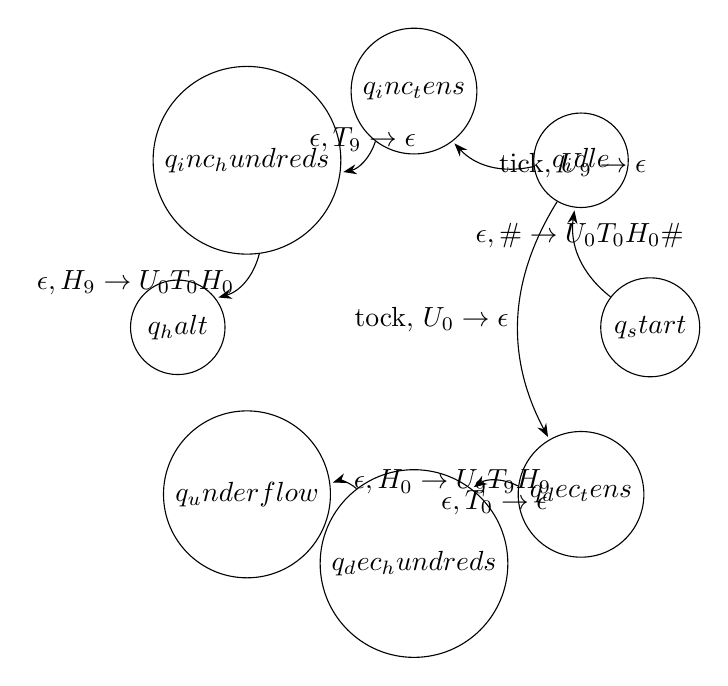
\begin{tikzpicture}[->, >=Stealth, shorten >=1pt, auto,
        node distance=2cm,
        state/.style={circle, draw, minimum size=1.2cm},
        every loop/.style={looseness=5},
      ]
      % place the 8 states on a circle
      \foreach \i/\name in {
        0/q_start, 45/q_idle, 90/q_inc_tens, 135/q_inc_hundreds,
        180/q_halt, 225/q_underflow, 270/q_dec_hundreds, 315/q_dec_tens}
        \node[state] (\name) at (\i:3cm) {$\name$};
  
      % Transitions (only key ones shown; you can add more)
      \draw (q_start) edge[bend left] node[above] {$\epsilon,\#\to U_0T_0H_0\#$} (q_idle);
      \draw (q_idle) edge[bend left] node[right] {tick, $U_9\to\epsilon$} (q_inc_tens);
      \draw (q_inc_tens) edge[bend left] node[above] {$\epsilon,T_9\to\epsilon$} (q_inc_hundreds);
      \draw (q_inc_hundreds) edge[bend left] node[left] {$\epsilon,H_9\to U_0T_0H_0$} (q_halt);
  
      \draw (q_idle) edge[bend right] node[left] {tock, $U_0\to\epsilon$} (q_dec_tens);
      \draw (q_dec_tens) edge[bend right] node[below] {$\epsilon,T_0\to\epsilon$} (q_dec_hundreds);
      \draw (q_dec_hundreds) edge[bend right] node[right] {$\epsilon,H_0\to U_9T_9H_9$} (q_underflow);
    \end{tikzpicture}
    \caption{Circular Layout of the Extended Up/Down (0–999) DPDA}
  \end{figure}\end{document}